%!TEX root = ../main.tex
\section{System Requirements} % (fold)
\label{sec:system_requirements}

\martin{The big system picture should be on its own page}

\begin{figure}[!h]
\centering
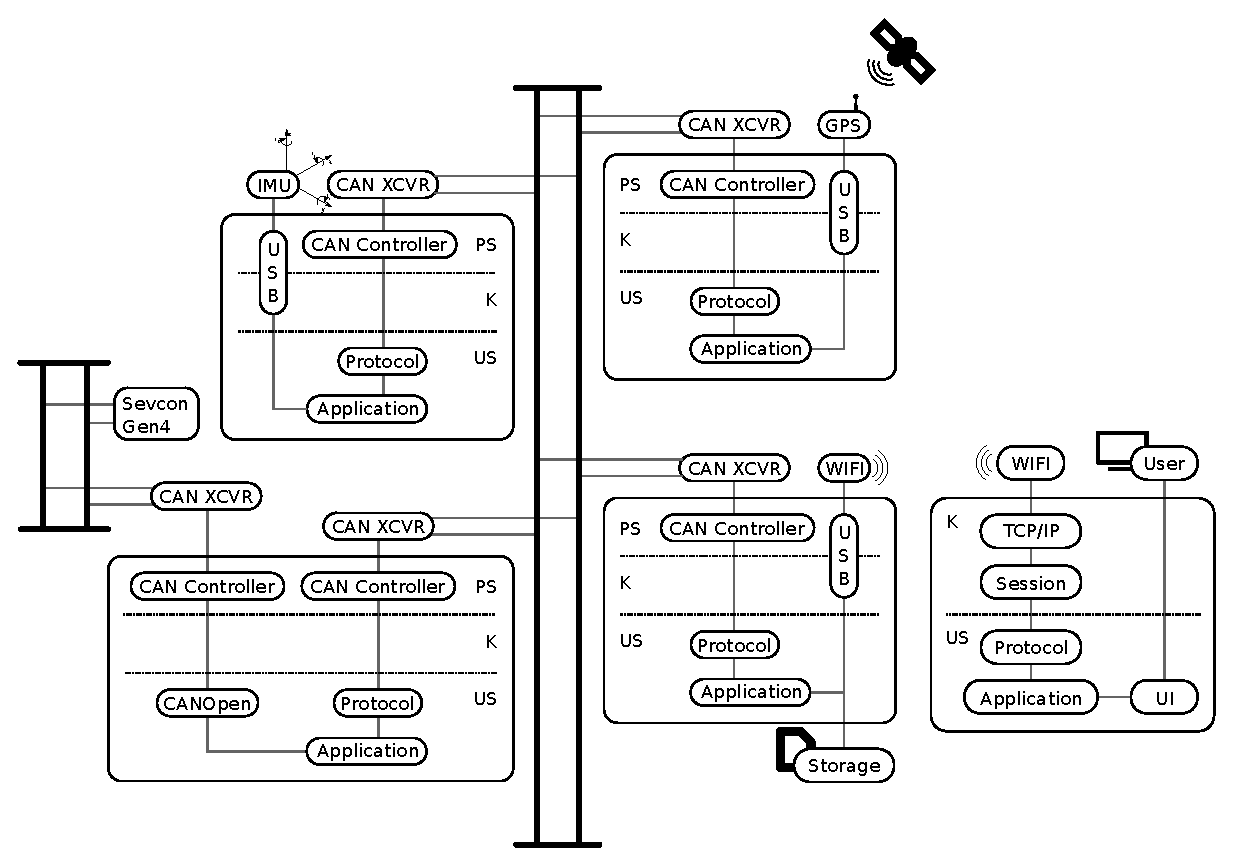
\includegraphics[angle=90,width=\textwidth]{graphics/analysis_complex.eps}
\caption{The big system........}
\label{fig:complete_system}
\end{figure}









\begin{tabular}{ |p{3cm}| }
\hline
\multicolumn{1}{|c|}{\textbf{Interfaces}}\\
\hline
USB \\
5V 3A PSU \\
Wifi \\
CAN \\
CANOpen \\
SD-card \\
\hline
\end{tabular}


\begin{table}[]
\centering
\caption{System requirements}
\label{tab:requirements}
\begin{tabular}{ |p{0.3cm}|p{8.5cm}|p{1cm}| }
\hline
\multicolumn{3}{|c|}{\textbf{Functional}}\\
\hline
1 & Read data from sensors/data producers 				& page x \\
2 & Timestamps all data 								& page x \\
3 & Transmit data wireless between Zybo board and pc 	& page x \\
4 & Log data to SD card 								& page x \\
5 & Transfer logs to pc 								& page x \\
6 & Start/stop transmission from nodes 					& page x \\
7 & Present data to user								& page x \\
8 & Provide an API for data access						& page x \\
9 & Must continue to function on node failure			& page x \\

\hline
\multicolumn{3}{|c|}{\textbf{Operational}}\\
\hline	
10 & A developer can add new nodes 						& page 1 \\
11 & A developer can modify existing nodes 				& page 1 \\
12 & A user can start/stop data transmission from nodes	& page 1 \\
13 & A user can request a data log 						& page 1 \\
14 & A developer can add API for specific sensor 		& page 1 \\
15 & A developer can add custum (G)UI					& page 1 \\


\hline
\multicolumn{3}{|c|}{\textbf{Quality of Service}}\\
\hline	
16 & Can support 16 nodes							 	& page 1 \\
17 & Has wireless range of 80 m						 	& page 1 \\
18 & CAN network has 1 Mb/s data bandwidth			 	& page 1 \\
19 & Timestamps with a precision of x ms 			 	& page 1 \\

\hline
\multicolumn{3}{|c|}{\textbf{Design}}\\
\hline	
20 & Must allow for integration of new nodes		 					& page 1 \\
21 & Software must be modular to allow for simple integration of nodes	& page 1 \\

\hline
\end{tabular}

\end{table}

% \subsection{Actors}
% The only actor on the system is an engineer.

% \subsection{Interfaces}
% \begin{itemize}
% \item Wifi, for data transfer between go-kart and stationary computer.
% \item CAN bus, for local network.
% \item CanOpen, for interfacing the Sevcon.
% \item USB, for GPS and IMU.
% \item ??, for SD card connection.
% \item Powersupply, for Zybo boards.
% \end{itemize}

% \subsection{Functional requirements}
% The system: 
% \begin{itemize}
% \item Reads data from sensors.
% \item Reads data from Sevcon.
% \item Transfers data to stationary computer using Wifi.
% \item Presents data to the user.
% \item Logs sensordata to SD card.
% \item Read data from SD card.
% \item Timestamps all data. 
% \end{itemize}

% \subsection{Operational requirements}
% The system monitors go-kart data.% when engineer starts the system by powering it on.

% \subsection{Quality of service requirements}
% \begin{itemize}
% \item IMU data must be sampled with xx Hz.
% \item GPS data must be sampled with zz Hz.
% \item Data logging with qq Hz.??
% \end{itemize}

% \subsection{Parametric requirements}
% Wifi range must be greater than xx meters.

% \subsection{Design requirements}
% The system:
% \begin{itemize}
% \item must be scalable to at least 16 sensors/nodes.
% \item must be modular to allow easy integration of new sensors/nodes.
% \item must be functional if one or more sensors/nodes stop working.	 
% \end{itemize}


% section system_requirements (end)